\section{Signal Extraction}
%%%%%%%%%%%%%%%%%%%%%%%%%%%%%%%%%%%%%%%%%%%%%%%%%%%%%%%%%%%%%%%%%%%%%%
\label{sec:SignalExtraction}
The signal is extracted in each bin of \pth by using a 2D template for signals and backgrounds in the \mll-\mt plane. This is the same strategy used in the main WW analysis. 
The binning of the \mll and \mt templates is:
\begin{itemize}
\item {\mll: $[12,30,45,60,75,100,125,150,175,200]$} 
\item {\mt: $[60,70,80,90,100,110,120,140,160,180,200,220,240,280]$}
\end{itemize}
We have checked that these two variables are not correlated with \pth, as shown in Fig.~\ref{fig:correlation_ggH} and Fig.~\ref{fig:correlation_vbf} for gluon fusion and VBF signals respectively.
\begin{figure}[htb]
\centering
\subfigure[]{\includegraphics[width=0.45\textwidth]{images/correlationmll_ggH.pdf}}
\subfigure[]{\includegraphics[width=0.45\textwidth]{images/correlationmth_ggH.pdf}}
\caption{Correlation between $\pth$ and $\mll$ (a) and between \pth and \mt (b) after the full selection for the gluon fusion signal.\label{fig:correlation_ggH}}
\end{figure}

\begin{figure}[htb]
\centering
\subfigure[]{\includegraphics[width=0.45\textwidth]{images/correlationmll_vbf.pdf}}
\subfigure[]{\includegraphics[width=0.45\textwidth]{images/correlationmth_vbf.pdf}}
\caption{Correlation between \pth and \mll (a) and between \pth and \mt (b) after the full selection for the VBF signal.\label{fig:correlation_vbf}}
\end{figure}

The signal extraction is performed using the {\tt combine} tool. 
We have defined a model with six signal strength parameters, one for each bin.
The relative contribution for different production mechanisms in the input signal template is taken to be the same as the SM.
The signal strength in each bin is allowed to float between -10 and +10, thus allowing negative values. This is mainly intended to allow the error bars to float below 0.\\
The fake events, i.e. reconstructed events not belonging to the fiducial region, are included in the signal definition. In fact in this step we are extracting all the events passing the analysis selection, regardless of the fiducial region definition.
Those events must be subtracted before the unfolding: to do this, given the fiducial region, we have computed the expected spectrum of fake events in bins of \pth. Then each bin of the spectrum is multiplied by the measured signal strength in that bin and then subtracted from the measured spectrum.
At the end, the number of events in each bin $i$ of the measured spectrum is:
\begin{equation}
N_i = \mu_i (s_i -f_i) \quad ,
\end{equation}
where $s_i$ and $f_i$ are respectively the number of signal and fake events expected from MC and $\mu_i$ is the measured signal strength.

\subsection{Fitting procedure}\label{subsec:fit}
The fit is a binned likelihood fit. Each source of systematic uncertainty is represented by a nuisance parameter in the fit.
Each signal is splitted in the six different bins of \pth as shown also in the yields table \ref{table:yields}. The WW and Top backgrounds have been also splitted in the various bins of Higgs \pt in order to reduce a possible shape mismatching between data and MC.\\
The fit is not performed on data, being the analysis is still blinded, but rather on a toy Asimov dataset. The best fit parameters values and the related profile-likelihood uncertainties extracted from the fit including all the nuisances in the model are shown in table \ref{table:fit_full}. For each parameter of interest the MINOS algorithm has been used.

\begin{table}
\centering
\caption{Best fit values and profile-likelihood uncertainties for all the signal strengths obtained fitting all the nuisances in the model.}\label{table:fit_full}
\begin{tabular}{c|c|c}
\hline
Signal strength & Best fit value & Uncertainty (68\% C.L.)\\
\hline\hline
$\mu_0$ & 1.000 & -0.408/+0.421 \\
$\mu_1$ & 1.000 & -0.294/+0.305 \\
$\mu_2$ & 1.000 & -0.420/+0.441 \\
$\mu_3$ & 1.000 & -0.860/+0.913 \\
$\mu_4$ & 1.001 & -1.224/+1.380 \\
$\mu_5$ & 1.001 & -0.932/+1.091 \\
\hline
\end{tabular}
\end{table}

In order to assess the robustness of the fit we have also run on several toy MC with a statistics corresponding to the one expected in data. The distribution of the signal strengths extracted in each bin in the toys and the their pulls are shown in Fig.~\ref{fig:pull_fit}. 
\begin{figure}[htb]
\centering
\subfigure[]{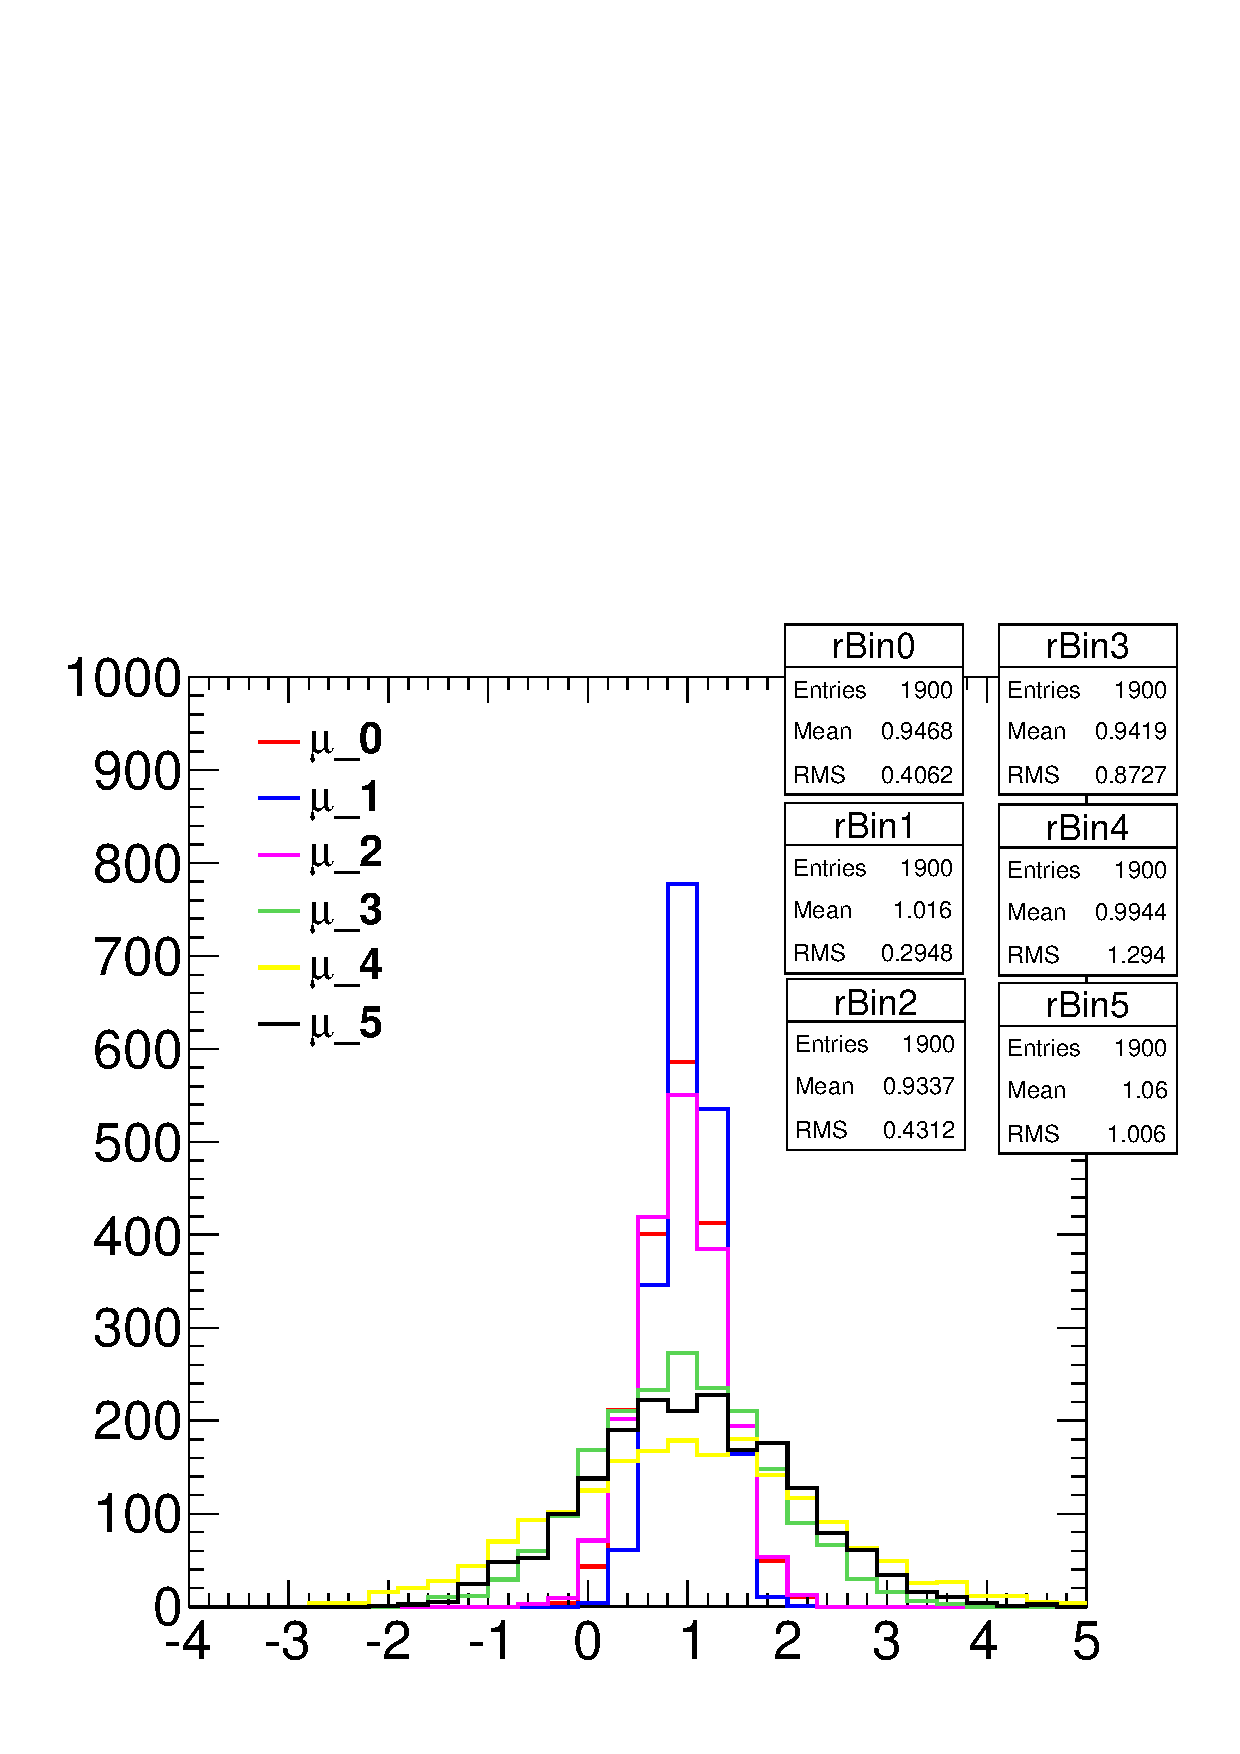
\includegraphics[width=0.45\textwidth]{images/mu_toys.pdf}}
\subfigure[]{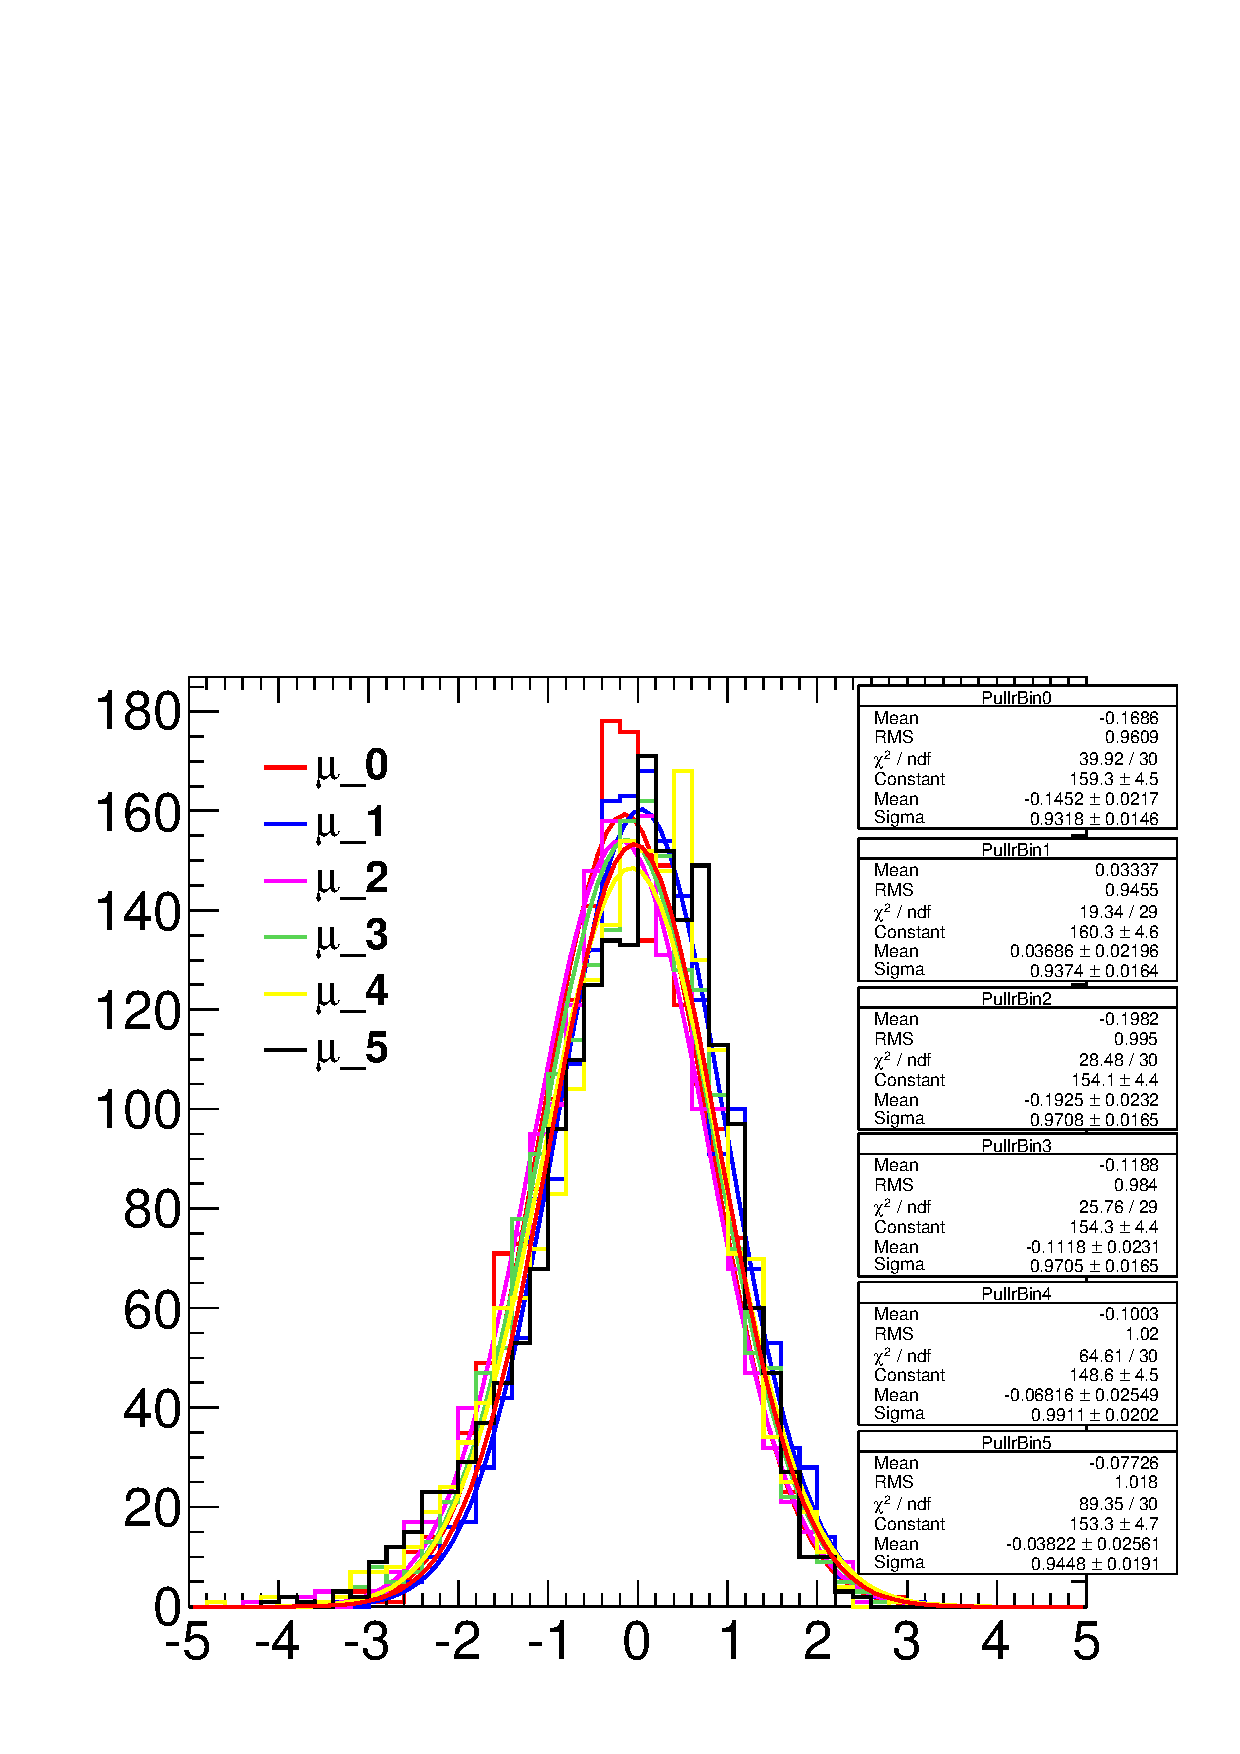
\includegraphics[width=0.45\textwidth]{images/pull_toys.pdf}}
\caption{Signal strengths distribution as extracted from the fit in toy MC (a). Pulls of the signal strength parameters (b).\label{fig:pull_fit}}
\end{figure}
